% Fig. 2 v3 (paper concept figure): three-layer physical hierarchy with the
% COMPLETE heat path as explicit nodes (DomainExpert model-ruling XVI).
%
% Upper panel (2.5D): die ->(ubump)-> interposer (explicit node, own temp
% field) ->(C4)-> substrate (explicit node) -> ambient; plus the heatsink
% branch die ->(TIM/lid)-> heatsink ->(convection)-> ambient. Every branch
% annotated with physical path type (conduction/convection/boundary) and
% value provenance. Cross-layer coupling constraints C1-C4 annotated.
% Lower panel (3D, model-ruling XIV): expanded per-layer dies + TSV
% inter-layer edge + lumped R_vert annotation. All routing orthogonal;
% sans-serif.
%
% Sources: config/thermal YAML values + thermal-module-catalog formulas;
% per-segment numeric values not fabricated.
\documentclass[border=10pt]{standalone}
\usepackage{sfmath}
\renewcommand{\familydefault}{\sfdefault}
\usepackage{tikz}
\usetikzlibrary{arrows.meta, shapes.geometric}
\definecolor{diefill}{HTML}{E8F0FE}
\definecolor{dieedge}{HTML}{1A73E8}
\definecolor{ipfill}{HTML}{F3E8FD}
\definecolor{ipedge}{HTML}{9334E6}
\definecolor{subfill}{HTML}{FFF4E5}
\definecolor{subedge}{HTML}{B45309}
\definecolor{hsfill}{HTML}{E0F2F1}
\definecolor{hsedge}{HTML}{00695C}
\definecolor{bndfill}{HTML}{F1F3F4}
\definecolor{bndedge}{HTML}{5F6368}
\definecolor{segsub}{HTML}{1A73E8}
\definecolor{seghs}{HTML}{B45309}
\definecolor{cbxfill}{HTML}{FFFFFF}
\definecolor{cbxedge}{HTML}{5F6368}
\begin{document}
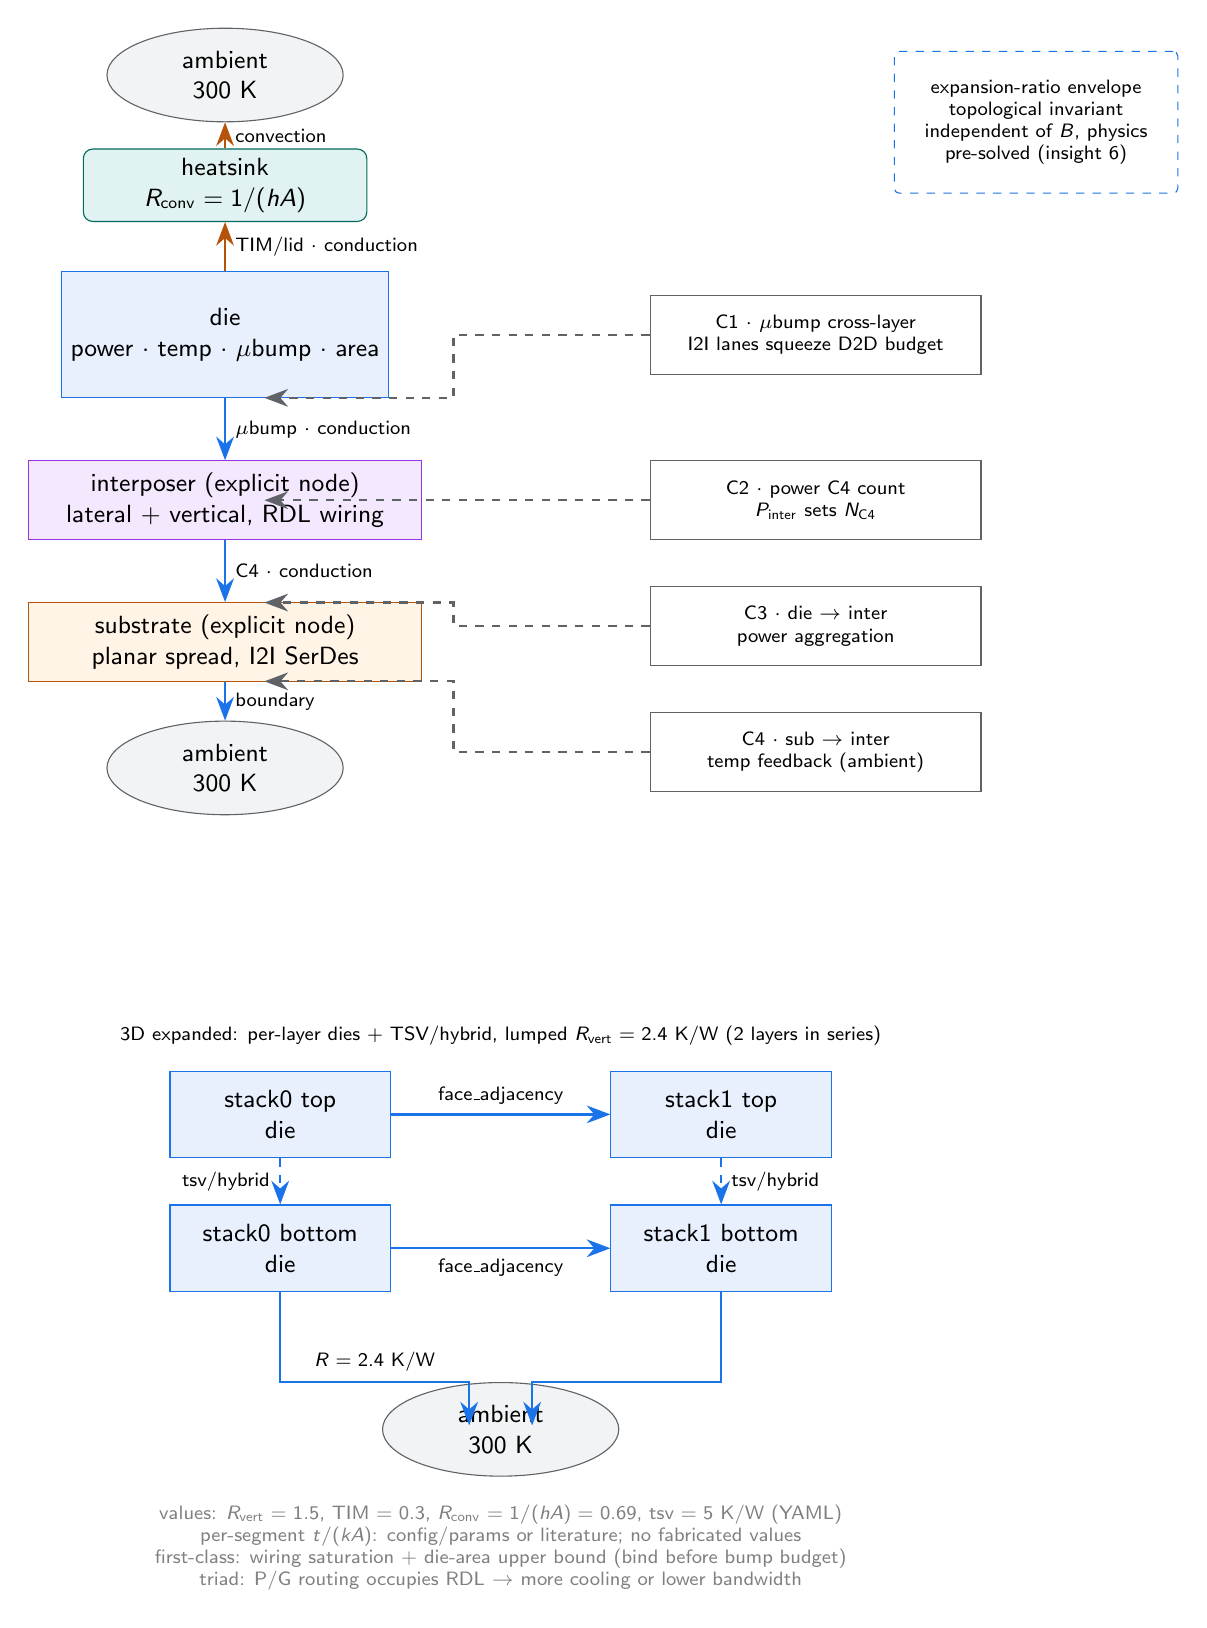
\begin{tikzpicture}[
  die/.style={rectangle, draw=dieedge, fill=diefill, minimum width=3.4cm,
              minimum height=1.6cm, align=center, font=\small},
  lnode/.style 2 args={rectangle, draw=#1, fill=#2, minimum width=5.0cm,
              minimum height=1.0cm, align=center, font=\small},
  hs/.style={rectangle, rounded corners=0.12cm, draw=hsedge, fill=hsfill,
             minimum width=3.6cm, minimum height=0.8cm, align=center, font=\small},
  bnd/.style={ellipse, draw=bndedge, fill=bndfill, minimum width=3.0cm,
              minimum height=1.0cm, align=center, font=\small},
  cbox/.style={rectangle, draw=cbxedge, fill=cbxfill, minimum width=4.2cm,
              minimum height=1.0cm, align=center, font=\scriptsize},
  segsub/.style={draw=segsub, thick, -{Stealth[length=3mm]}},
  seghs/.style={draw=seghs, thick, -{Stealth[length=3mm]}},
  cpl/.style={draw=cbxedge, thick, -{Stealth[length=3mm]}, dashed},
  lab/.style={font=\scriptsize},
]
% ================= UPPER PANEL: 2.5D complete chain (left column) ==========
\node[die] (die) at (-3.5, 13.5) {die\\power $\cdot$ temp $\cdot$ $\mu$bump $\cdot$ area};
\node[hs] (heatsink) at (-3.5, 15.4) {heatsink\\$R_{\mathrm{conv}}=1/(hA)$};
\node[bnd] (ambient_hs) at (-3.5, 16.8) {ambient\\300 K};
\node[lnode={ipedge}{ipfill}] (interposer) at (-3.5, 11.4) {interposer (explicit node)\\lateral + vertical, RDL wiring};
\node[lnode={subedge}{subfill}] (substrate) at (-3.5, 9.6) {substrate (explicit node)\\planar spread, I2I SerDes};
\node[bnd] (ambient) at (-3.5, 8.0) {ambient\\300 K};
% segments with branch annotation (physical type + value provenance)
\draw[seghs] (die.north) -- node[right, lab] {TIM/lid $\cdot$ conduction} (heatsink.south);
\draw[seghs] (heatsink.north) -- node[right, lab] {convection} (ambient_hs.south);
\draw[segsub] (die.south) -- node[right, lab] {$\mu$bump $\cdot$ conduction} (interposer.north);
\draw[segsub] (interposer.south) -- node[right, lab] {C4 $\cdot$ conduction} (substrate.north);
\draw[segsub] (substrate.south) -- node[right, lab] {boundary} (ambient.north);
% ================= C1-C4 coupling boxes (right) =============================
\node[cbox] (c1) at (4.0, 13.5) {C1 $\cdot$ $\mu$bump cross-layer\\I2I lanes squeeze D2D budget};
\node[cbox] (c2) at (4.0, 11.4) {C2 $\cdot$ power C4 count\\$P_{\mathrm{inter}}$ sets $N_{\mathrm{C4}}$};
\node[cbox] (c3) at (4.0, 9.8) {C3 $\cdot$ die $\rightarrow$ inter\\power aggregation};
\node[cbox] (c4) at (4.0, 8.2) {C4 $\cdot$ sub $\rightarrow$ inter\\temp feedback (ambient)};
\draw[cpl] (c1.west) -- (-0.6, 13.5) |- (-3.0, 12.7);   % -> die/ubump level
\draw[cpl] (c2.west) -- (-0.6, 11.4) -- (-3.0, 11.4);    % -> interposer
\draw[cpl] (c3.west) -- (-0.6, 9.8) -- (-0.6, 10.1) -- (-3.0, 10.1);  % -> inter-sub
\draw[cpl] (c4.west) -- (-0.6, 8.2) -- (-0.6, 9.1) -- (-3.0, 9.1);    % -> substrate
% envelope side box (insight 6)
\node[draw=dieedge, dashed, rounded corners=0.06cm, fill=white,
      minimum width=3.6cm, minimum height=1.8cm, align=center, font=\scriptsize] (env) at (6.8, 16.2)
      {expansion-ratio envelope\\topological invariant\\independent of $B$, physics\\pre-solved (insight 6)};
% ================= LOWER PANEL: 3D expanded (model-ruling XIV) ==============
\node[draw=dieedge, fill=diefill, minimum width=2.8cm, minimum height=1.1cm,
      align=center, font=\small] (t0) at (-2.8, 3.6) {stack0 top\\die};
\node[draw=dieedge, fill=diefill, minimum width=2.8cm, minimum height=1.1cm,
      align=center, font=\small] (b0) at (-2.8, 1.9) {stack0 bottom\\die};
\node[draw=dieedge, fill=diefill, minimum width=2.8cm, minimum height=1.1cm,
      align=center, font=\small] (t1) at (2.8, 3.6) {stack1 top\\die};
\node[draw=dieedge, fill=diefill, minimum width=2.8cm, minimum height=1.1cm,
      align=center, font=\small] (b1) at (2.8, 1.9) {stack1 bottom\\die};
\node[bnd] (amb3d) at (0, -0.4) {ambient\\300 K};
\draw[segsub, dashed] (t0.south) -- node[left, lab] {tsv/hybrid} (b0.north);
\draw[segsub, dashed] (t1.south) -- node[right, lab] {tsv/hybrid} (b1.north);
\draw[segsub] (t0.east) -- node[above, lab] {face\_adjacency} (t1.west);
\draw[segsub] (b0.east) -- node[below, lab] {face\_adjacency} (b1.west);
\draw[segsub] (b0.south) -- (-2.8, 0.2) -- node[above, lab] {$R=2.4$ K/W} (-0.4, 0.2) -- (-0.4, -0.35);
\draw[segsub] (b1.south) -- (2.8, 0.2) -- (0.4, 0.2) -- (0.4, -0.35);
\node[lab, align=center] at (0, 4.6) {3D expanded: per-layer dies + TSV/hybrid, lumped $R_{\mathrm{vert}}=2.4$ K/W (2 layers in series)};
% ================= provenance note (incl. first-class + triad semantics) ====
\node[lab, align=center, text=gray] at (0, -1.9) {
  values: $R_{\mathrm{vert}}=1.5$, TIM $=0.3$, $R_{\mathrm{conv}}=1/(hA)=0.69$, tsv $=5$ K/W (YAML)\\
  per-segment $t/(kA)$: config/params or literature; no fabricated values\\
  first-class: wiring saturation + die-area upper bound (bind before bump budget)\\
  triad: P/G routing occupies RDL $\rightarrow$ more cooling or lower bandwidth};
\end{tikzpicture}
\end{document}
